\documentclass[runningheads]{llncs}

\usepackage[T1]{fontenc}
\usepackage{graphicx}
\usepackage{hyperref}

% If you use the hyperref package, please uncomment the following two lines
% to display URLs in blue roman font according to Springer's eBook style:
\usepackage{color}
\renewcommand\UrlFont{\color{blue}\rmfamily}
\urlstyle{rm}

%----Making things more compact
\newcommand{\smalltt}[1]{\small \texttt{#1}}
\newenvironment{packed_itemize}{
\vspace*{-0.2em}
\begin{itemize}
\setlength{\partopsep}{0pt}
\setlength{\itemsep}{1pt}
\setlength{\parskip}{0pt}
\setlength{\parsep}{0pt}
}{\end{itemize}}
\newenvironment{packed_enumerate}{
\vspace*{-0.2em}
\begin{enumerate}
\setlength{\partopsep}{0pt}
\setlength{\itemsep}{1pt}
\setlength{\parskip}{0pt}
\setlength{\parsep}{0pt}
}{\end{enumerate}}
\renewcommand{\textfraction}{0.07}
\renewcommand{\topfraction}{0.9}
\renewcommand{\bottomfraction}{0.9}
\renewcommand{\floatpagefraction}{0.66}
\setlength{\floatsep}{2.0pt plus 2.0pt minus 2.0pt}
\setlength{\textfloatsep}{5.0pt plus 2.0pt minus 0.0pt}
\title{SUMO-ML-NLP: A Neuro-Symbolic Question Answering System}
\titlerunning{SUMO-ML-NLP}
\author{
Adam Pease\inst{1}\orcidID{0000-0001-9772-1266} \and
Roberto Milanese\inst{1}\orcidID{0009-0009-5107-162X} \and
Jarrad Singley\inst{1}\orcidID{0009-0009-7640-3782} \and
Richard Thompson\inst{1}\orcidID{0009-0001-6541-1092} \and
Angelos Toutisios\inst{1}\orcidID{0009-0009-6064-5154} \and
Geoff Sutcliffe\inst{2}\orcidID{0000-0001-9120-3927}}

\authorrunning{A. Pease et al.}

\institute{Naval Postgraduate School, Monterey, USA \\
\email{\{adam.pease,roberto.milanese,jarrad.singley,richard.thompson,angelos.toutsios.gr\}@nps.edu}\\
\and
University of Miami, Miami, USA \\
\email{geoff@cs.miami.edu}}

\begin{document}
\maketitle              % typeset the header of the contribution
%--------------------------------------------------------------------------------------------------
\begin{abstract}
The abstract should briefly summarize the contents of the paper in
150--250 words.

\keywords{First keyword  \and Second keyword \and Another keyword.}
\end{abstract}
%--------------------------------------------------------------------------------------------------
\section{Introduction}
\label{Introduction}

SUMO-ML-NLP is a tool chain that uses Machine Learning (ML) for translation of natural language to 
logic, Automated Theorem Proving (ATP) to reason about the logic, and Natural Language Processing
(NLP) to translate the results of the reasoning to natural language.
SUMO-ML-NLP is unique in that it leverages the rich SUMO ontology~\cite{Pea11} and supporting
infrastructure~\cite{PB10-IKBET} to provide
background knowledge for the translations.

WHY ARE THESE IMPORTANT OR USEFUL?

The use of deductive technique for question answering is a well known quest, harking back
to early work by Bert Green et al.~\cite{GW+61}.
Purely deductive efforts were also evident early in the development of question answering
systems, e.g.,~\cite{GR68,Gre69}, and later work includes~\cite{FG+08,SYT09}, with significant
community effort evident~\cite{GCW10}.
Purely NLP-based approaches include~\cite{WHAT}.
Approaches that integrate deduction with NLP include~\cite{JS24}.
Recent advances in generative language systems have made question answering directly possible
based on data learned from the internet and other large corpora, 
e.g.,~\cite{Ope23,TM+23,Gem23}, sometimes augmented by domain-specific content in 
retrieval-augmented generation systems, e.g.,\cite{Cha22}.
As results from purely generative systems can be erroneous~\cite{Hallucinations}, using
symbolic reasoning, deductive reasoning in particular, to verify the generated answers, is
a rich field of research~\cite{HMS24}.
Work closest to SUMO-ML-NLP are with the use of the Cyc ontology~\cite{CMB05}, the 
Inquire Biology knowledge base~\cite{CC+13}, and use of provenance information in answering
semantic web queries\cite{MP04}.

The complete architecture of SUMO-ML-NLP is shown in Figure~\ref{ArchitecturePicture}, and the
details of the various compoments are given in Sections~\ref{Training}~and~\ref{Running}.

In step 1 of Figure \ref{fig:arch} a user enters a statement or question in natural language that is passed in step 2 to a component (based on OLLaMa) that attempts to detect whether any metaphors are present and then attempts to translate them to a literal reading if so.
In step 3 the result of metaphor rephrasing is passed to a component that attempts to simplify complex sentences into a set of shorter and simpler sentences.  It is also based around OLLaMa.  We also use the Stanford Stanza system to recognize co-references (such as pronouns) and replace them with the most meaningful token from the original sentence.  For example, if presented with the sentence ``John went to the store and he bought cookies.'' simplification might generate ``John went to the store.'', ``He bought cookies.''  We process sentences one at a time so ``He'' would not be meaningful.  Instead, we replace ``He'' with ``John''.

Since there are a potentially infinite set of things like people and place names that will not be present in our training data set, we try to recognize words and phrases that are out of the training vocabulary (step 4).  We use the Stanford Stanza Named Entity Recognition (NER) system to find these words or phrases and guess at their types.  We have mapped the types to SUMO and use that to state the basic identity of the word or phrase.  For example, if we have ``John climbed Mt. St. Helens.'' NER should recognize ``Mt. St. Helens'' as a place, which would then be asserted as an instance of a SUMO \texttt{GeographicArea}.  We include a set of generic tags in our training data to cover unknown vocabulary, so we process the sentence into ``John climbs UNK-Region-1.''  We can then perform machine translation (step 5) to convert that language to logic as follows:

\begin{verbatim}
(exists (?J ?C ?R)
  (and
    (instance ?J Human)
    (names "John" ?J)
    (instance ?C Climbing)
    (located ?C UNK-Region-1)
    (agent ?C ?J)))
\end{verbatim}

post processing (step 6) replaces the unknown term and asserts its type

\begin{verbatim}
(instance MtStHelens GeographicArea)

(exists (?J ?C ?R)
  (and
    (instance ?J Human)
    (names "John" ?J)
    (instance ?C Climbing)
    (located ?C MtStHelens)
    (agent ?C ?J)))
\end{verbatim}

Finally, in step 7 these statements are combined with the existing content of SUMO.   If the user subsequently issues the command ``test'' to the system, then Vampire will attempt to find a contradiction among the previously asserted statements and SUMO and provide a detailed proof (step 8).  If the English input is a question then this will become a logical conjecture that Vampire attempts to prove.

We have an early (inactive) prototype in our pipeline that attempts to provide an English arguments instead of a mathematical proof.  It is currently deactivated but can be tested by uncommenting code in sumonlp/src/runpipeline.sh.

This SigmaNLP code \url{https://github.com/ontologyportal/sigmanlp}
generates language-logic pairs designed for training a machine learning system. Several approaches are used:

\begin{itemize}
\item instantiate relations with arguments of appropriate types and then generate NL paraphrases from them
\item run through all formulas in SUMO and generate NL paraphrases
\item build up sentences and logic expressions compositionally
\end{itemize}

%--------------------------------------------------------------------------------------------------
\section{Architecture}
\label{Architecture}

\begin{figure}
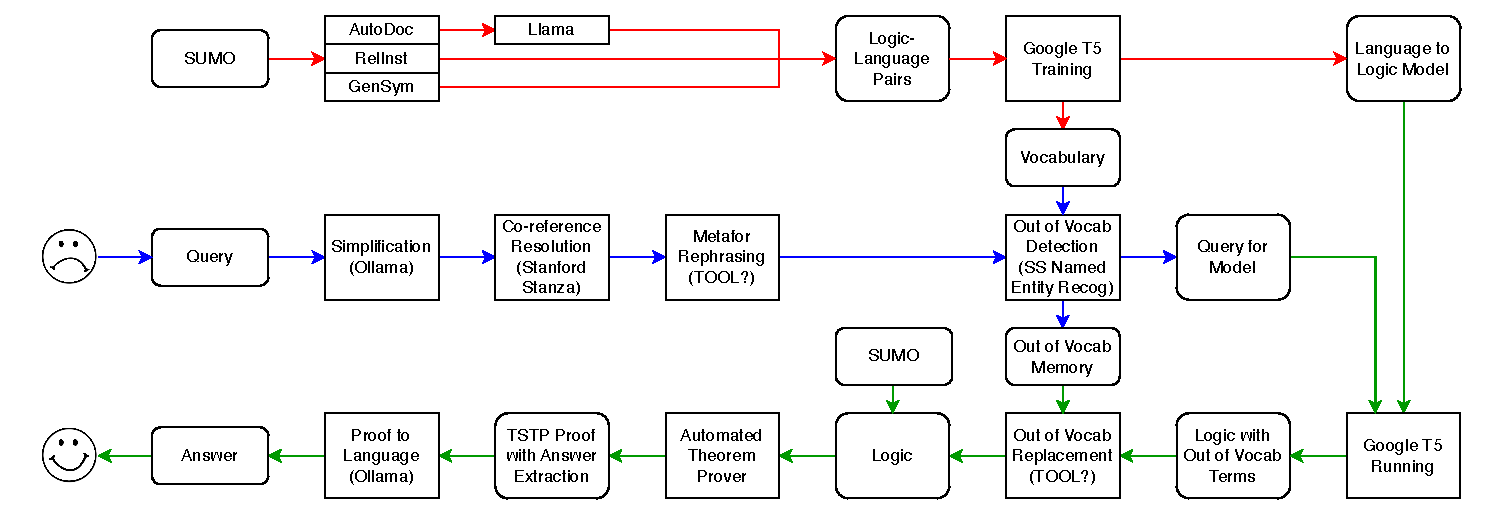
\includegraphics[width=\textwidth]{Architecture.pdf}
\caption{SUMO-ML-NLP architecture}
\label{ArchitecturePicture}
\end{figure}

GEOFF

%--------------------------------------------------------------------------------------------------
\section{Training the SUMO Model}
\label{Training}

ADAM

%--------------------------------------------------------------------------------------------------
\section{Running a Query}
\label{Running}

GEOFF

%--------------------------------------------------------------------------------------------------
\subsection{Building the Query}
\label{BuildingQuery}

ROBERTO

JARRAD

ANGELOS

%--------------------------------------------------------------------------------------------------
\subsection{Answering the Query}
\label{AnsweringQuery}

ANGELOS

ADAM

%--------------------------------------------------------------------------------------------------
\section{Conclusion}
\label{Conclusion}

%--------------------------------------------------------------------------------------------------
\bibliographystyle{splncs04}
\bibliography{Bibliography.bib}
%--------------------------------------------------------------------------------------------------
\end{document}
%--------------------------------------------------------------------------------------------------
